\documentclass[combined.tex]{subfiles}
\usepackage{amssymb}
\usepackage[spanish]{babel}
\pagestyle{plain}

\begin{document}

\chapter{Curriculum Vitae}

\begin{tabular}{c|c}
\begin{minipage}{10cm}
\name{Jorge Alda Gallo}
\vspace{0.8cm}
\presentation{Doctorado en Física Teórica}
\noindent
\email{jalda@unizar.es}
\phone{+34 676 70 35 11}
\address{C/Rioja 18 2B, 50017 Zaragoza, Spain.}
\webpage{https://jorge-alda.github.io}
\github{Jorge-Alda}
\orcid{0000-0002-6728-1105} 
\end{minipage} & \hspace{1cm} 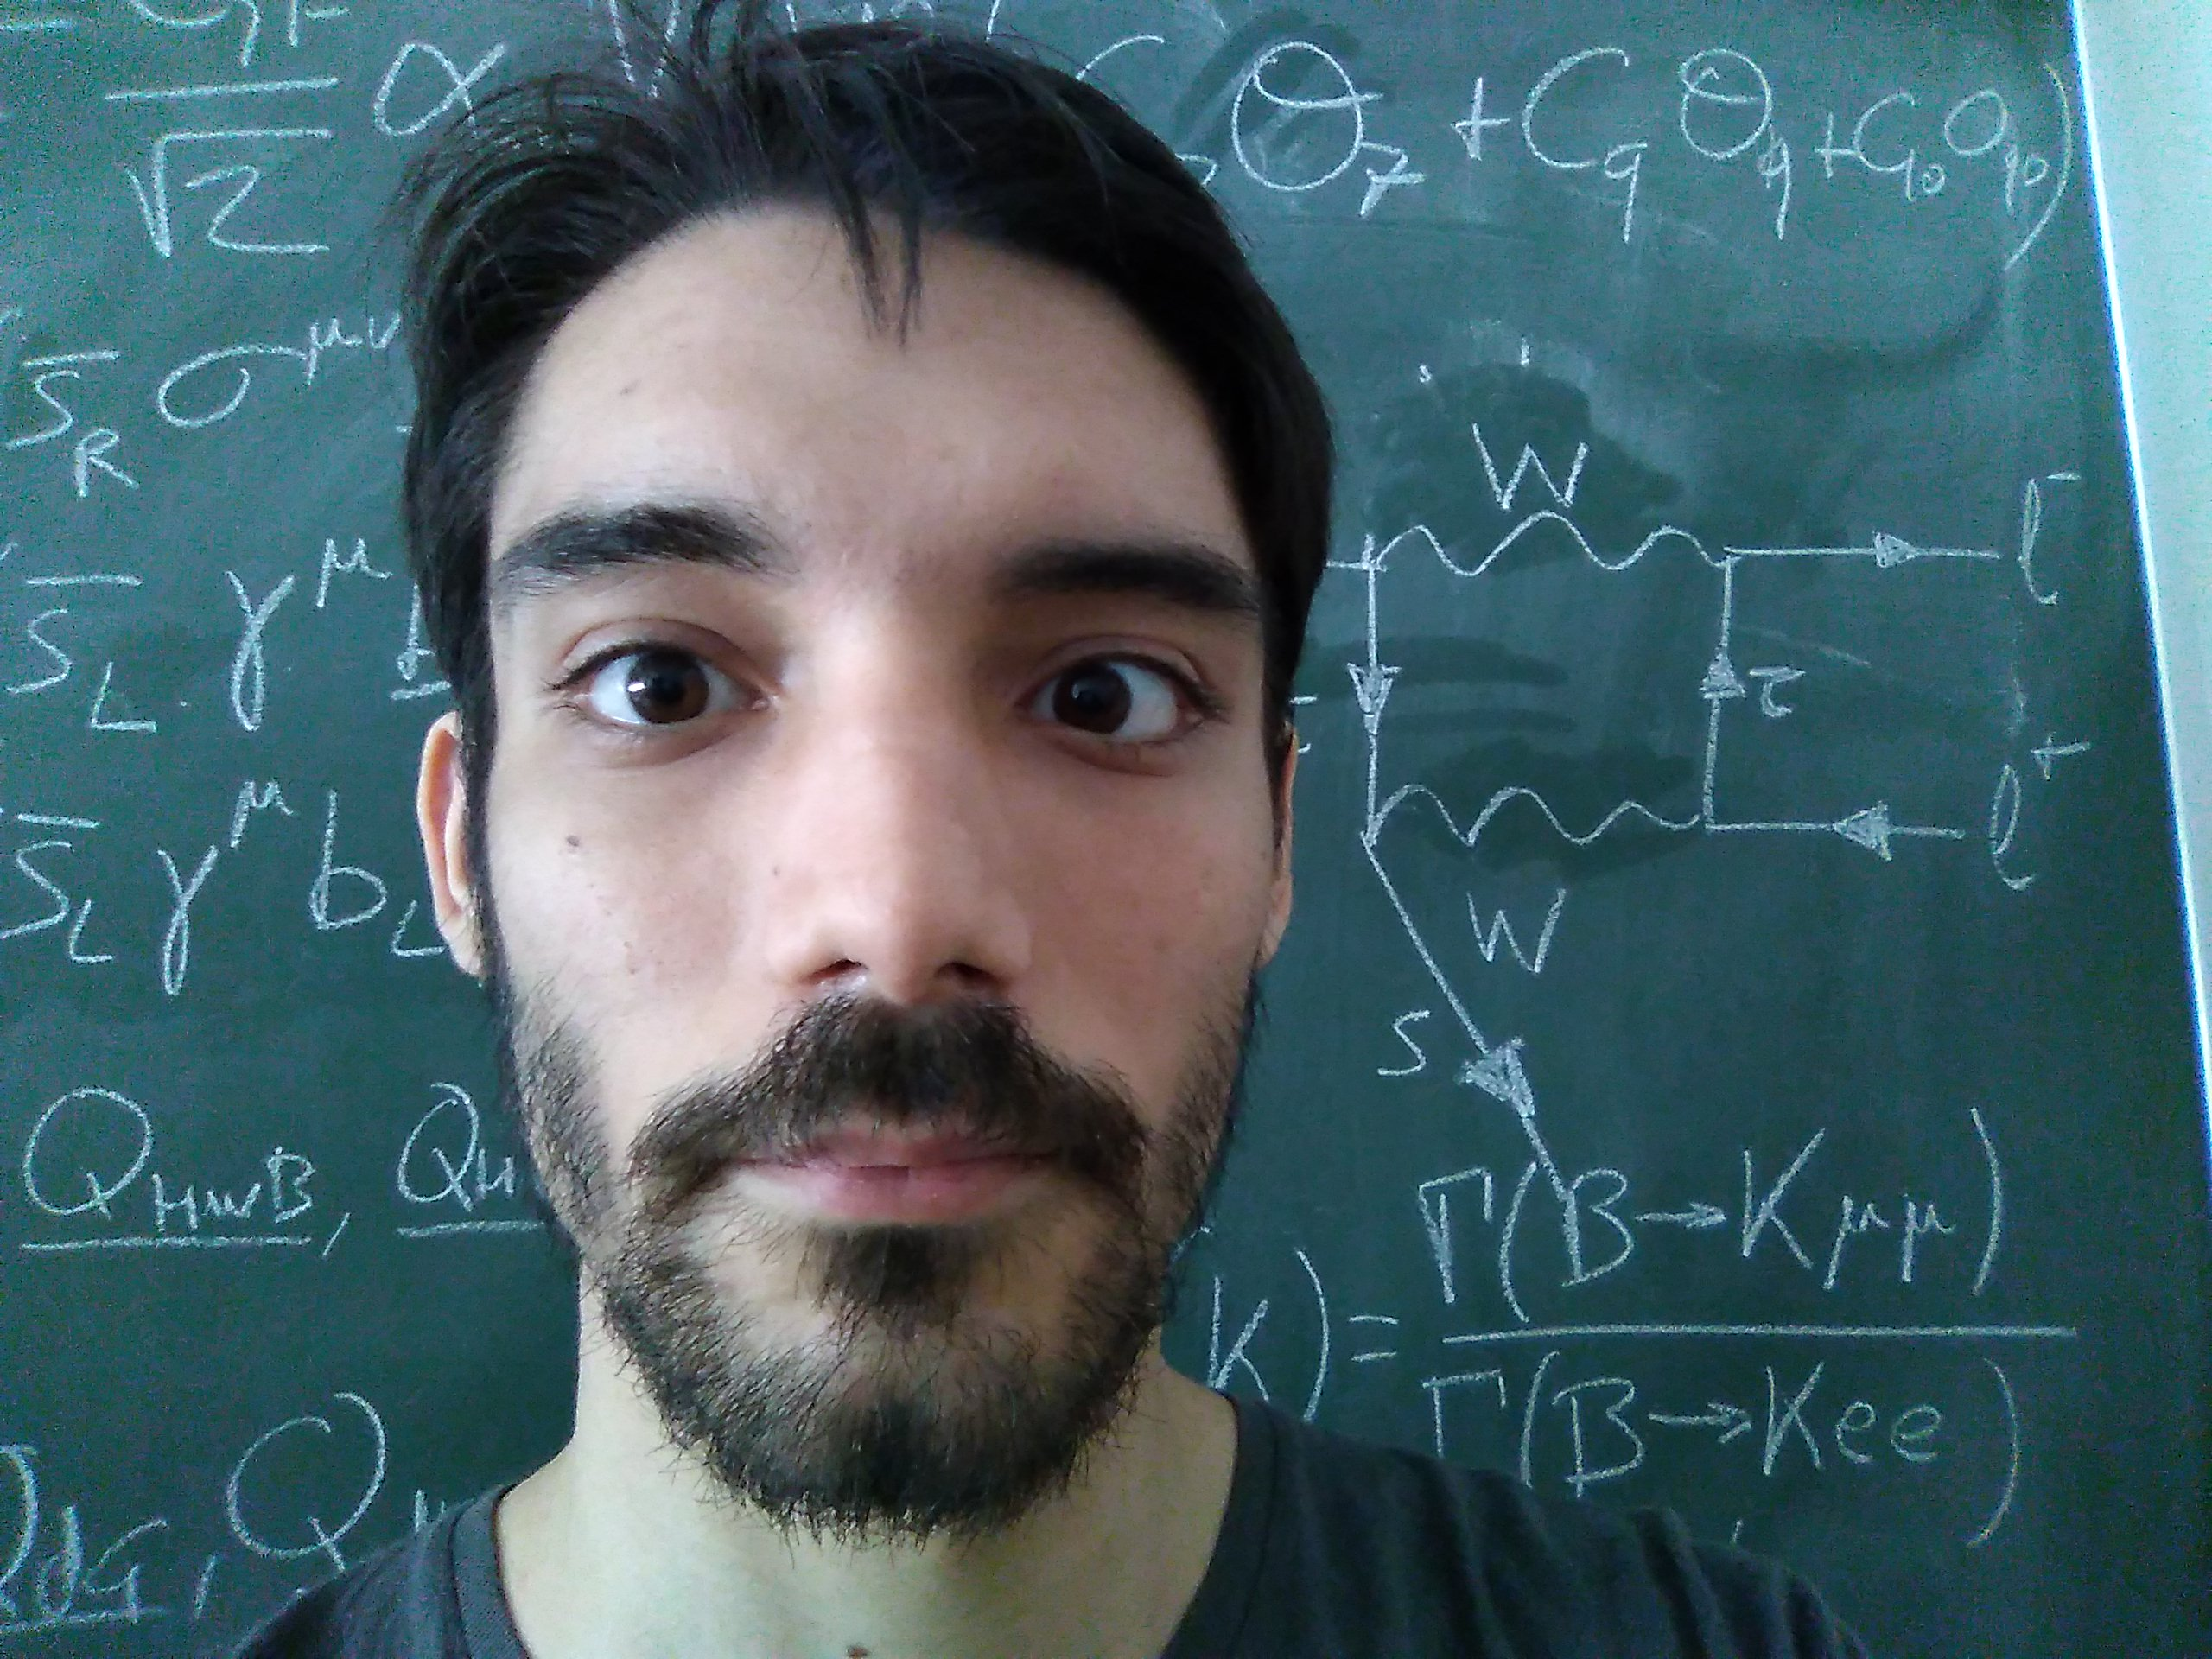
\includegraphics[width=4cm]{photo.jpg}
\end{tabular}

\interests{Intereses de investigación}
\begin{itemize}
\item Nueva Física más allá del Modelo Estándar.
\item Física del sabor.
\item Anomalías de los mesones $B$.
\item Teorías de Campos efectivas.
\item Axiones y ALPs
\end{itemize}

\education{Formación}
\datedsubsection{Grado en Física, Universidad de Zaragoza}{2011-2015}
Nota Media: 9.20/10. 13 Matrículas de Honor.\\
Trabajo de Fin de Grado: \textit{``Cálculo numérico en teoría cuántica de campos de la materia condensada''}. Bajo la supervisión de David Zueco Láinez. Calificación: 9.5/10.

\datedsubsection{Máster en Física Teórica, Universidad Complutense de Madrid}{2015-2016}
Nota Media: 9.34/10.\\
Trabajo de Fin de Máster: \textit{New Applications of the Coleman-Weinberg Model}. Bajo la supervisión de J. A. Ruiz Cembranos. Calificación: 9.0/10.

\datedsubsection{Escuela de Doctorado}{2018}
Taller de Altas Energías. Benasque (Huesca).

\datedsubsection{Doctorado en Física, Universidad de Zaragoza}{2016-2022}
Bajo la supervisión de Siannah Peñaranda Rivas.\\
Título de la tesis: \textit{A Glance into Flavour Physics with Effective Field Theories and Machine Learning}.

\grants{Becas y Contratos}
\datedsubsection{Beca JAE-Intro CSIC}{2014}
Proyecto \textit{``Caos semiclásico en sistemas de bosones con interacción''}, supervisado por David Zueco Láinez.\\
CSIC-ICMA (Instituto de Ciencia de Materiales de Aragón).

\datedsubsection{Contrato de Investigador Predoctoral, Diputación General de Aragón}{2017-2022}

\datedsubsection{Beca del Programa Ibercaja-CAI de Estancias de Investigación}{2021}
Beca No. CB 5/21.

\memberships{Pertenencia a instituciones científicas}
\datedsubsection{CAPA}{2019-presente}
Centro de Astropartículas y Física de Altas Energías. Zaragoza, Spain.\\
\url{capa.unizar.es}

\invited{Estancias de investigación}
\datedsubsection{Università degli Studi di Padova/INFN}{Junio-Septiembre 2021}

\works{Producción científica}

\hspace{\parindent}
\textbf{J. Alda, J. Guasch and S. Peñaranda: \textit{Some results on Lepton Flavour Universality Violation}}\\
Eur.Phys. J. C, 79 7 (2019) 588\\
doi:10.1140/epjc/s10052-019-7092-x\\
arXiv:1805.03636 [hep-ph]

~

\textbf{J. Alda, J. Guasch and S. Peñaranda: \textit{Anomalies in $B$ decays: A phenomenological approach}}\\
Eur.Phys. J. Plus 137 (2022) 217\\
doi:10.1140/epjp/s13360-022-02405-3\\
arXiv:2012.14799 [hep-ph]

~

\textbf{J. Alda, J. Guasch and S. Peñaranda: \textit{Anomalies in $B$ decays: Present status and future collider prospects}}\\
arXiv:2105.05095 [hep-ph]\\
SLAC eConf C21-03-15.1

~

\textbf{J. Alda, J. Guasch and S. Peñaranda: \textit{Using Machine Learning techniques in phenomenological studies in flavour physics}}\\
arXiv:2109.07405 [he-ph]

~

\textbf{J. Alda, J. Guasch and S. Peñaranda: \textit{Exploring B-physics anomalies at colliders}}\\
arXiv:2110.12240 [hep-ph]\\
PoS(EPS-HEP2021)494

~

\textbf{J. Alda, A. W. M Guerrera, S. Peñaranda and S. Rigolin: \textit{Leptonic Meson Decays into Invisible ALP}}\\
arXiv:2111.02536 [hep-ph]

\conferences{Charlas y conferencias}

\hspace{\parindent}\textbf{2nd Red LHC Workshop. Madrid. 9-11 Mayo 2018}\\
Charla ``Some Results on Lepton Flavour Violation''.

~

\textbf{Taller de Altas Energías. Benasque (Huesca) 2-15 Septiembre 2018}\\
Charla ``Some Results on Lepton Flavour Violation''.

~

\textbf{X CPAN Days. Salamanca. 29-31 Octubre 2018}\\
Charla ``Complex Wilson coefficients in the analysis of $B$-anomalies''.

~

\textbf{I Jornadas de Jóvenes Investigadores CAPA. Zaragoza. 7 Mayo 2019}\\
Charla ``Effective Theories for $B$-meson anomalies''.

~

\textbf{I Jornadas del Programa de Doctorado de Física. Zaragoza. 20 Junio 2019}\\
Charla ``Effective Theories for $B$-meson anomalies''.

~

\textbf{XXXVII Bienal de Física de la Real Sociedad Española de Física. Zaragoza. 15-19 de Julio 2019}\\
Chrala ``Some Results on Lepton Flavour Universality Violation''.

~

\textbf{International Workshop on Future Linear Colliders - LCWS2021. Online. 15-18 Marzo 2021}\\
Charla ``Anomalies in $B$ mesons decays: Present status and future collider prospects''.

~

\textbf{European Physical Society Conference on High Energy Physics 2021 (EPS-HEP2021). Online. 26-30 Julio 2021}\\
Póster ``Exploring B-physics anomalies at colliders ''.

~

\textbf{Seminario, Departmento de Física Teórica. Universidad de Zaragoza. 18 Noviembre 2021}\\
Charla ``Leptonic Mesons Decays into invisible ALP''.

~

\textbf{II Jornadas del Programa de Doctorado de Física. Universidad de Zaragoza. 3 Diciembre 2021}\\
Charla ``Leptonic Mesons Decays into invisible ALP''.

~

\textbf{Seminario, Departmento de Física Teórica. Universidad de Zaragoza. 20 Enero 2022}\\
Charla ``Using Machine Learning techniques in phenomenological studies in flavour physics''.

~

\textbf{Seminario, Instituto de Física Teórica (IFT). Universidad Autónoma de Madrid. 27 Enero 2022}\\
Charla ``Using Machine Learning techniques in phenomenological studies in flavour physics''.

\repositories{Contributiones a repositorios de código informático}

\subsection{flavio}
1 contribución incorporada: \url{https://github.com/flav-io/flavio/pull/160}

\subsection{smelli}
1 contribución: \url{https://github.com/smelli/smelli/pull/45}

\teaching{Docencia}

\subsection{Septiembre 2019}
\hspace{\parindent}\textbf{Escuela de Doctorado ``Taller de Altas Energías de Benasque'' (Huesca).}\\
Profesor asociado.

\subsection{2019-2020}
\hspace{\parindent}\textbf{Ecuaciones diferenciales}\\
Sesiones de problemas, 38 horas lectivas.\\
Segundo curso del Grado en Física, Universidad de Zaragoza.

~

\textbf{Física General}\\
Sesiones de laboratorio, 10 horas lectivas.\\
Primer curso del Grado en Matemáticas, Universidad de Zaragoza.

\subsection{2020-2021}
\hspace{\parindent}\textbf{Ecuaciones diferenciales}\\
Sesiones de problemas, 38 horas lectivas.\\
Segundo curso del Grado en Física, Universidad de Zaragoza.

~

\textbf{Física General}\\
Sesiones de laboratorio, 10 horas lectivas.\\
Primer curso del Grado en Matemáticas, Universidad de Zaragoza.

\subsection{2021-2022}
\hspace{\parindent}\textbf{Ecuaciones diferenciales}\\
Sesiones de problemas, 38 horas lectivas.\\
Segundo curso del Grado en Física, Universidad de Zaragoza.

~

\textbf{Co-dirección de Trabajo de Fin de Grado}\\
10 horas lectivas.
Cuarto curso del Grado en Física, Universidad de Zaragoza.


\languages{Idiomas}
\begin{tabular}{ll}
Inglés & \level{5} \\
Italiano & \level{3} \\
Alemán & \level{3} \\
Francés & \level{2}
\end{tabular}

\coding{Lenguajes de programación}
\begin{tabular}{ll}
\TeX/\LaTeX & \level{5}\\
Python & \level{5}\\
C/C++ & \level{3}\\
Mathematica & \level{3}
\end{tabular}

\awards{Premios}
\datedsubsection{XXII Olimpiada Española de Física}{2011}
Medalla de Plata (Puesto 15).\\
Segunda posición en la fase aragonesa.

\datedsubsection{20th International Mathematics Competition}{2013}
Medalla de Bronce (Puesto 177).

\newpage

\section{Acerca de este CV}
\begin{tabular}{L{10.5cm}C{5.5cm}}
\begin{minipage}[b]{10cm}
Este CV ha sido actualizado el día \today.\\
La versión más reciente está disponible en \\ \url{https://raw.githubusercontent.com/Jorge-Alda/CV/CV_ES/CV.pdf}
\end{minipage} & \includegraphics[width=3cm]{qrcode.png}
\end{tabular}


\end{document}